\documentclass[12pt]{article}
\usepackage[margin=1in]{geometry}
\usepackage{amsmath,amssymb,amsthm,booktabs,graphicx,natbib,microtype}
\newtheorem{theorem}{Theorem}
\newtheorem{corollary}[theorem]{Corollary}
\newtheorem{remark}[theorem]{Remark}
\title{Optimal Gram-Gauge Pairing\\\large Ordered Generalized Eigenframes and the Tail-Inflation Barrier}
\author{Prime Dynamics Theory Program}
\date{July 2026}

\begin{document}
\maketitle

\begin{abstract}
RH-120 transfers a relative tail constant through any gauge satisfying two
Loewner comparisons, but leaves the gauge choice open.  We solve the exact
recent-Gram problem.  Let $G,G'\succ0$, $D,D'\succ0$, and let
$\alpha_1\leq\cdots\leq\alpha_4$ and
$\beta_1\leq\cdots\leq\beta_4$ be the generalized eigenvalues of $(D,G)$
and $(D',G')$.  Among all $S$ satisfying $S^*GS=G'$, the least $b$ for which
$D'\preceq bS^*DS$ is
\[
 b_{\rm opt}=\max_i\frac{\beta_i}{\alpha_i}.
\]
It is attained by aligning the ordered generalized eigenframes.  A
96-pair five-scale audit has zero theorem failures, but exposes a finite
barrier: only 25 pairs have $b_{\rm opt}<1$, the median is $27.6936$, and a
weak-direction mismatch produces a conditioned maximum near
$9.88\times10^{290}$.  Thus exact recent-Gram alignment is optimally solved
but does not by itself supply a uniform physical recurrence.
\end{abstract}

\section{The minimax gauge problem}
For a positive pair $(G,D)$ define its relative tail matrix
\[
 A=G^{-1/2}DG^{-1/2}.
\]
The squared RH-114 Rayleigh constant is $\lambda_{\max}(A)$.  Given a target
pair $(G',D')$, RH-120 asks for $a,b,S$ such that
$G'\succeq aS^*GS$ and $D'\preceq bS^*DS$.  We first impose exact recent
alignment, $S^*GS=G'$, so $a=1$, and minimize the remaining tail factor.

Every exact-Gram gauge has the form
\begin{equation}\label{eq:gauge}
 S=G^{-1/2}UG'^{1/2},\qquad U^*U=I.
\end{equation}
Indeed, \eqref{eq:gauge} gives exact alignment, and conversely
$U=G^{1/2}SG'^{-1/2}$ is unitary.  With
$B=G'^{-1/2}D'G'^{-1/2}$, the tail comparison becomes
\begin{equation}\label{eq:relative}
 B\preceq bU^*AU.
\end{equation}

\section{Optimal ordered-eigenframe theorem}
\begin{theorem}[Optimal exact-Gram gauge]\label{thm:optimal}
Let $A,B\succ0$ have ascending eigenvalues
$\alpha_1\leq\cdots\leq\alpha_n$ and
$\beta_1\leq\cdots\leq\beta_n$.  Then
\[
 \min_{U^*U=I}\ \inf\{b:B\preceq bU^*AU\}
 =\max_{1\leq i\leq n}\frac{\beta_i}{\alpha_i}.
\]
An optimizer maps an ordered eigenbasis of $B$ to the correspondingly
ordered eigenbasis of $A$.
\end{theorem}
\begin{proof}
If \eqref{eq:relative} holds, monotonicity of ordered Hermitian eigenvalues
gives $\beta_i\leq b\alpha_i$ for every $i$; hence every unitary has
$b\geq\max_i\beta_i/\alpha_i$.  Choose eigenvector matrices $V_A,V_B$ and
set $U=V_AV_B^*$.  Then
$U^*AU=V_B\operatorname{diag}(\alpha_i)V_B^*$, while
$B=V_B\operatorname{diag}(\beta_i)V_B^*$.  The comparison holds exactly for
$b=\max_i\beta_i/\alpha_i$.
\end{proof}
The only external ingredients are standard congruence calculus and ordered
eigenvalue monotonicity \citep{Bhatia2007,HornJohnson1991}.

Combining Theorem~\ref{thm:optimal} with RH-120 yields
\[
 \gamma'\leq\sqrt{b_{\rm opt}}\,\gamma.
\]
The induced gamma bound need not be sharp because the ratio attaining
$b_{\rm opt}$ may occur below the top generalized mode.  It is sharp when
the maximal ordered ratio occurs at an index also determining the source
top eigenvalue.

\begin{corollary}[Semidefinite obstruction]
In the limiting semidefinite problem, if some ordered source value
$\alpha_i$ is zero while $\beta_i>0$, no finite exact-Gram tail factor can
exist.
\end{corollary}
This is the mechanism behind very large conditioned values: a direction
that is nearly invisible to the source tail can carry non-negligible target
tail energy.

\section{Finite five-scale pairing audit}
We recompute the RH-114 packet-block Gramians on the five archived scales.
Adjacent scales are paired by side, threshold, and four normalized phases,
giving $4\times2\times3\times4=96$ pairs.  To make the generalized pencils
numerically definite, both recent and tail Gramians receive an explicitly
recorded relative $10^{-12}$ spectral floor after outward PSD correction.
This defines a regularized finite diagnostic; it is not silently treated as
a lower support certificate.

For every pair we construct the ordered-eigenframe gauge, verify exact Gram
alignment, verify the Loewner tail upper, compare both Rayleigh constants,
and enumerate all 24 eigenvalue permutations.  There are zero failures in
all four categories.  The scale-edge results are
\begin{table}[h]
\centering
\begin{tabular}{lrrr}
\toprule
edge & pairs with $b_{\rm opt}<1$ & median $b_{\rm opt}$ & maximum $b_{\rm opt}$\\
\midrule
$0.16\to0.08$ & 4/24 & $3.3753\times10^4$ & $9.88\times10^{290}$\\
$0.08\to0.04$ & 3/24 & $1.0863\times10^5$ & $3.69\times10^8$\\
$0.04\to0.02$ & 15/24 & 0.881856 & 230.059\\
$0.02\to0.01$ & 3/24 & 27.4686 & $4.2721\times10^4$\\
\bottomrule
\end{tabular}
\caption{Finite optimal tail inflation.  The enormous first-edge maximum is
a conditioned weak-mode diagnostic, not an asymptotic claim.}
\end{table}

Across all pairs, 25 are contractive, the median is 27.693586, and every
target regularized gamma remains below one.  The optimal transferred upper
is often loose because a lower generalized direction, rather than the top
one, controls $b_{\rm opt}$.

\begin{figure}[h]
\centering
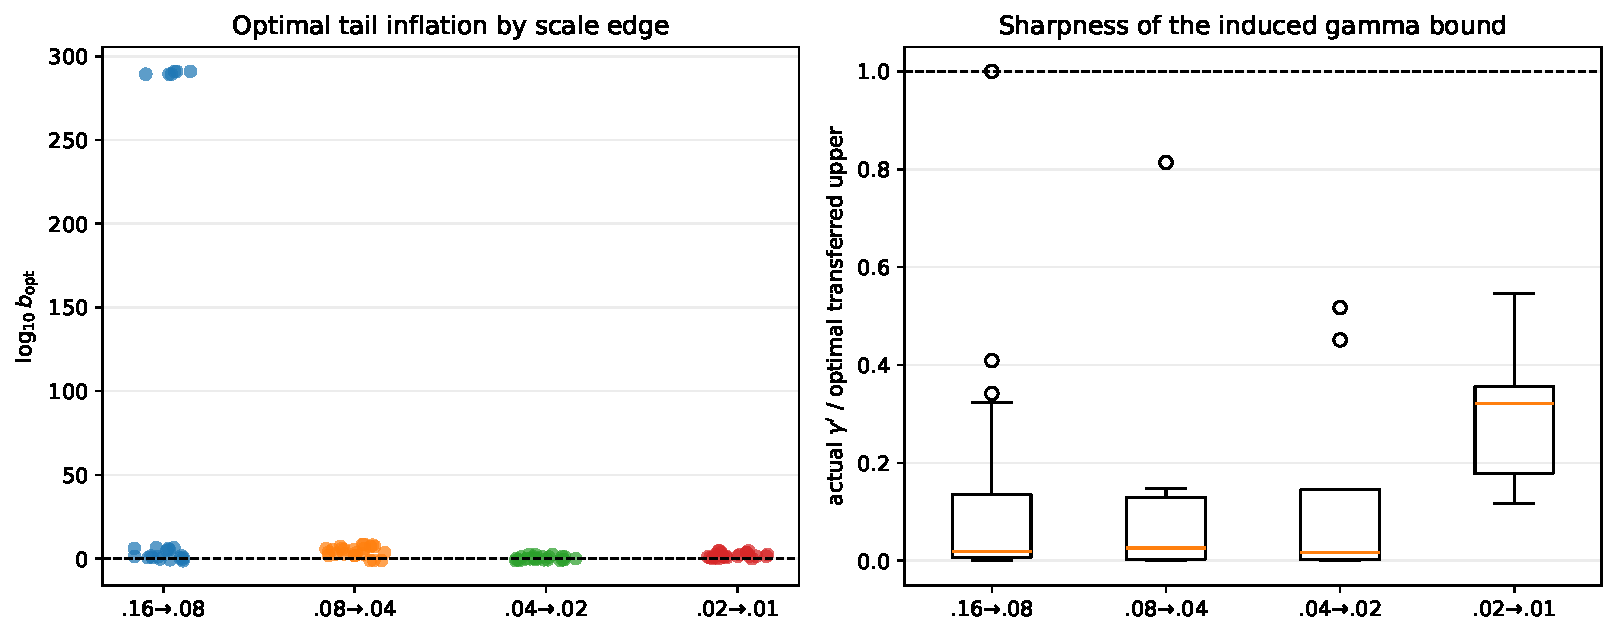
\includegraphics[width=\textwidth]{figures/optimal_gram_gauge_pairing.pdf}
\caption{Left: intrinsic exact-Gram tail inflation.  Right: efficiency of
the resulting gamma upper.}
\end{figure}

\section{What is closed and what remains}
The gauge-choice problem is closed at the exact finite-dimensional level:
no different exact alignment can beat the ordered generalized-spectrum
formula.  The audit also gives a useful negative answer to a tempting next
step.  Recent-Gram alignment alone does not produce a small or monotone tail
factor on the archived chain.  A physical recurrence must control the whole
relative pair, permit explicit defects, or exploit additional dynamics.

RH-122 isolates the still sharper fixed-coordinate obstruction.  RH-123
then allows additive Loewner defects, which is the form needed for outward
transport.  No finite extrema above are extrapolated to all scales.  No
uniform Stage A, Hilbert--Polya operator, zeta-zero identification, or
Riemann Hypothesis conclusion is claimed.

\bibliographystyle{plainnat}
\bibliography{references}
\end{document}
